\documentclass[article,nojss,shortnames]{jss}

\usepackage{thumbpdf,lmodern}
\usepackage{framed}
\usepackage{algorithmic}
\usepackage{amsmath}
\usepackage[]{algorithm2e}

\newcommand{\note}[1]{\textcolor{red}{\textbf{Note:} #1}}


% Draft
%\hypersetup{draft}
%\shortcites{rasmussen2012}

\author{Reto Stauffer\\Universit\"at Innsbruck
\And Matthias Dusch\\Universit\"at Innsbruck
\AND Fabien Maussion\\Universit\"at Innsbruck
\And Georg J. Mayr\\Universit\"at Innsbruck}

\Plainauthor{Reto Stauffer, Matthias Dusch, Fabien Maussion, Georg J. Mayr}

\title{phoeton: Software for Objective Probabilistic Foehn Classification}
\Plaintitle{phoeton: Objective Probabilistic Foehn Classification}
\Shorttitle{phoeton: Objective Probabilistic Foehn Classification}

\Abstract{
    This is the abstract here \dots
}

\Keywords{meteorology, foehn, objective classification, flexible mixture model}
\Plainkeywords{meteorology, foehn, objective classification, flexible mixture model}

\Address{
  Reto Stauffer\\
  Department of Statistics\\
  Faculty of Economics and Statistics\\
  Universit\"at Innsbruck\\
  Universit\"atsstr.~15\\
  6020 Innsbruck, Austria\\
  E-mail: \email{Reto.Stauffer@uibk.ac.at}\\
  URL: \url{https://retostauffer.org}\\

  Matthias Dusch, Fabien Maussion, Georg J. Mayr\\
  Department of Atmospheric and Cryospheric Sciences\\
  Faculty of Geo- and Atmospheric Sciences\\
  Universit\"at Innsbruck\\
  Innrain~52f\\
  6020 Innsbruck, Austria\\
  E-mail: \email{Georg.Mayr@uibk.ac.at},
          \email{Matthias.Dusch@uibk.ac.at},
          \email{Fabien.Maussion@uibk.ac.at}
}


\begin{document}

% -------------------------------------------------------------------
% SECTION: INTRODUCTION
% -------------------------------------------------------------------
\section{Introduction}

Introduction why this is so great. Georg might like to contribute
here. Just to leave/include some references:
\begin{itemize}
    \item finite mixture model \citep{leisch2004,gruen2008}
    \item automatic probabilistic foehn classification \cite{plavcan2014}
    \item IWLS/IRLS \citep{mccullagh1989}
    \item Community foehn classification experiment \cite{mayr2018unpublished}
\end{itemize}

I would go for something like:

Gap winds are typically characterized by strong increase of wind speed with a rapid
rise in temperature and a drop in relative humidity during the onset. Such winds can be
found in various regions on our globe and bear different names for specific
regions such as the Santa-Anna winds in California which became infamous due to
their destructive effect in combination with wild fires, the Chinook winds in
the Rocky Mountain area, Mistral and Bora in south France and Croatia, or the
Foehn winds in the European Alps.  Over the past decades \textit{foehn} wind
has become a synonym for such gap flows and will be used in this article.
However, the method as presented is applicable for all gap flow winds
independent from their geographical location.

The conceptual model of foehn winds is quite well known
\citep{armi2007,mayr2008,armi2011}, however, foehn cannot measured directly.
Historically, foehn was often diagnosed manually by looking at available
meteorological records such as wind speed and direction, time series of
temperature and humidity, the conditions of the sky (e.g., occurrence of
lenticularis clouds in the region), and observations upstream and downstream of
the location of interest.  Some of the longest records of foehn observations
can be found in Switzerland (Altdorf \note{i'm just guessing!}) reaching back
to 1850 (\note{just guessing!}) for a hand full of stations.  These records are
typically based on manual classification made by experienced weather observers,
weather enthusiasts, and meteorologists.  This task is very time consuming and
is only done for some selected sites, typically sites with long historical
records. To be able to extend the diagnosis and to perform foehn classification
on a large number of meteorological sites, computer aimed classification is
needed.

Few attempts to automatically classify foehn winds have been proposed over the
past years such as \note{cite this and that}. These methods are mostly binary
(either \textit{yes} or \textit{no}) and require manual tuning to specify the
hyper-parameters, e.g., thresholds used to classify a specific observation as
foehn. \cite{plavcan2014} proposed a new automated probabilistic foehn
classification method based on finite mixture models, a statistical
regression-based model for automatic foehn classification. In a recent study of
\cite{mayr2018unpublished} this new method has been tested against existing
classification methods and manual foehn classification made by students and
experts to proof the diagnostic power of the new approach.

Overall, the automatic finite mixture model based foehn classification
\citep{plavcan2014} is able to compete with the human classification
\citep{mayr2018unpublished} and has the advantages that it is (i) reproducible,
and (ii) can easily be applied to large volumes of data. This allows one to
efficiently perform foehn classification for a wide range of different sites.

The article by \citep{plavcan2014} introduced the method using a powerful
package called \code{FlexMix} \citep{leisch2004,gruen2007,gruen2008} available
for the statistical software \textit{R}.  However, only little guidance was
given by \citep{plavcan2014} on how to apply this method to own data and an
implementation of the method outside the \textit{R} programming language was
not available until today.  Thus, the aim of this article is to introduce the
algorithm behind the automated probabilistic foehn classification
\citep{plavcan2014} in more detail and introducing new open-source software for
\textit{R} and \textit{Python} which provides the required methods to perform
the classification.  Furthermore, the software comes with a set of examples and
diagnostic tools for this specific task which allows everyone to use the method
on their own.

Section~\ref{sec:methods} describes the method itself followed by
Section~\ref{sec:software}  introducing the software with a set of
examples. Section~\dots \note{case study? Required for this article?}


% -------------------------------------------------------------------
% SECTION: METHODS
% -------------------------------------------------------------------
\section{Methods}\label{sec:methods}

\textit{Note by Reto:}
The original publication (\code{FlexMix}, \citealt{gruen2008})
provides general framework for flexible mixture models for multiple
components. For this application we will concentrate on the special
case with only two distinct components ($K = 2$).

Thus, this section introduces a simplified approach to estimate 
a finite mixture model for the special case with two distinct
Gaussian distributions and a binomial logit model to estimate
the coefficients for the concomitant variables.

\note{\dots ... and so far, and so on.}

\subsection{Finite mixture models}

Finite mixture models are a general model class of finite
mixtures of regression models. It is assumed that the mixture
consists of a set of $K$ distinct components, each described by
a parametric distribution.
In addition, an weight is assigned to each of the $K$ classes
for each observation which describes the a-priori probability
for an observation to come from this component.
These weights can depend on multiple covariates which are
referred to as \textit{concomitant} variables.

\begin{equation}
    h(\mathit{y} | \mathit{x}, \mathit{\omega}, \mathit{\alpha}, \mathit{\theta}) =
        \sum_{k=1}^K \pi_k(\mathit{\alpha}, \mathbf{\omega}) \cdot f_k(\mathit{y} | \mathit{x}, \mathit{\theta}_k)
        ~~\text{for}~~k=1,\dots,K
    \label{eqn:flexmix-density-general}
\end{equation}

where $\mathit{\theta}$ and $\mathit{\alpha}$ denote the parameters for the
mixture density $h()$. $\mathit{y}$ denotes the response, $\mathit{x}$ the
predictor variable (one single variable) and $\mathbf{\omega}$ the concomitant
variables for the probability model.

For the special case of a finite mixture model with $K=2$ Gaussian components
the specification as shown in Equation~\ref{eqn:flexmix-density-general} simplifies to

\begin{equation}
    h(\mathit{y} | \mathit{x}, \mathit{\omega}, \mathit{\alpha}, \mathit{\theta}) =
        \underbrace{
            (1 - \mathit{\pi}(\mathbf{\omega}, \mathit{\alpha})) \cdot
            \phi(\mathit{y} | \mathit{\theta}_1, \mathit{x})
        }_{\text{component 1}}
        \cdot
        \underbrace{
            \mathit{\pi}(\mathbf{\omega}, \mathit{\alpha}) \cdot \phi(\mathit{\theta}_2|\mathit{x})
        }_{\text{component 2}}
    \label{eqn:flexmix-density-gaussian}
\end{equation}

where $\phi()$ is the probability function of the Gaussian distribution.
The concomitant model for $\pi()$ reduces to a binomial problem as the probability
for a specific observation $y_i$ to be observed in the first component is the
counter probability of $y_i$ being observed in the second component.
Thus, for $\pi()$ any type of binomial model can be used which satisfies
that $\pi \in [0,1] \forall i=1,\dots,N$.
Figure~\ref{fig:schematic_density} shows an example of a finite mixture model with
two Gaussian components with fixed $\mathit{\theta}$ coefficients but different
weights or a-priori probabilities $\tilde{p}_k$.


\begin{figure}[h]
    \centering
    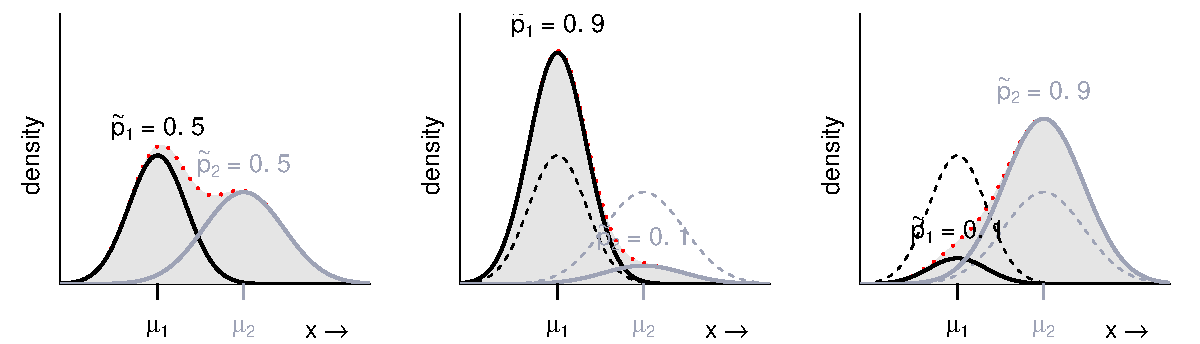
\includegraphics[width = .8\textwidth]{draft_schematic_density}
    \caption{Schematic representation of the finite mixture model density
    (shaded; red dashed line) and the two Gaussian components (black/gray). 
    $\tilde{p}_1$ and $\tilde{p}_2$ are the a-prior weights for the components.
    The dashed lines always show the distribution of the component with equal
    and constant weights of $\tilde{p}_1 = \tilde{p}_2 = 0.5$.}
    \label{fig:schematic_density}
\end{figure}

One frequently used model for a binary response is the binomial logistic regression
model or binomial logit model (BLM), however, any appropriate binomial probability
model could be used for $\pi$.
The BLM is defined as follows:

\begin{equation}
    \log\Big(\frac{\pi}{1 - \pi}\Big) =
        \omega^\top \alpha = \alpha_0 + \omega_1 \alpha_1 + \dots + \omega_P \alpha_P,
\end{equation}

where $\mathit{\pi}$ is the probability that an observation belongs to the
second component (Eqn.~\ref{eqn:flexmix-density-gaussian}).
The probabilities are modelled using multilinear regression
$\mathit{\omega}^\top \mathit{\alpha}$ with $p=1,\dots,P$ concomitant
variables $\mathit{\omega}$ times the corresponding parameters or regression
coefficients $\mathit{\alpha}$.

As the BLM is a generalized linear model, the parameters can be estimated using
an iterative (re-)weighted least squares (IWLS) solver.
The IWLS procedure to estimate the parameters $\mathit{\alpha}$ of the BLM
is shown in Algorithm~\ref{alg:iwls}.

\begin{algorithm}
    \caption{Iterative (re-)weighted least squares (IWLS) solver for the binomial logit model (BLM).}
    \label{alg:iwls}

    \textbf{Initialization ($j = 0$):}
    \begin{enumerate}
        \item Initialize $\mathit{\alpha}^{0} = 0$.
        \item Compute initial latent response $\mathit{\eta}^{(0)} = \mathbf{\omega}^\top\mathit{\alpha}^{(0)}$.
        \item Compute initial probabilities $\pi^{(0)} = \frac{\exp(\eta^{(0)})}{1 + \exp(\eta^{(0)})}$. 
        \item Evaluate initial log-likelihood:
            \begin{equation*}
                \ell^{(0)} = %(\mathit{\alpha} | \mathbf{\omega})^{(0)} =
                \sum_{i=1}^{N} \Big(\log(1 - \pi_i^{(0)})^{(y_i = 0)} + \log(\pi_i)^{(y_i=1)}\Big)
            \end{equation*}

    \end{enumerate}
    \textbf{Iterative parameter estimation ($j = 1, \dots, J$):}
    \begin{enumerate}
        \item Compute new inverse square root weights:
            \begin{equation*}
                \mathit{W}^{(j)} = \Big(\big(\frac{d\eta}{d\pi}\big)^{(j-1)}\Big)^{-\frac{1}{2}} =
                    \big(\mathit{\pi}^{(j-1)} (1 - \mathit{\pi}^{(j-1)})\big)^\frac{1}{2}
            \end{equation*}
        %%%\item Compute new latent response:
        %%%    \begin{equation*}
        %%%        \mathit{z}^{(j+1)} = \mathit{\eta}^{(j)} + (\mathit{y} - \mathit{\pi}^{(j)})
        %%%            \Big(\frac{d \mathit{\eta}}{d \mathit{\pi}}\Big)^{(j)} =
        %%%            \mathit{\eta}^{(j)} + \frac{\mathit{y} - \mathit{\pi}^{(j)}}{\mathit{\pi}^{(j)}(1 - \mathit{\pi}^{(j)})}
        %%%    \end{equation*}
        \item Update parameters:
            \begin{equation*}
                \mathit{\alpha}^{(j)} =
                    \big((\mathbf{\omega} \mathit{W}^{(j)})^\top
                    (\mathbf{\omega} \mathit{W}^{(j)})\big)^{-1}
                    (\mathbf{\omega} \mathit{W}^{(j)})^\top
                    \mathit{W}^{(j)} \mathit{z}^{(j)}
            \end{equation*}

            with $\mathit{z}^{(j)} = \mathit{\eta}^{(j-1)} + (\mathit{y} - \mathit{\pi}^{(j-1)}) \Big(\frac{d\pi}{d\eta}\Big)^{(j-1)}$ this yields

            \begin{equation*}
                \mathit{\alpha}^{(j)} =
                    \big((\mathbf{\omega} \mathit{W}^{(j)})^\top
                    (\mathbf{\omega} \mathit{W}^{(j)})\big)^{-1}
                    (\mathbf{\omega} \mathit{W}^{(j)})^\top
                    \Big(\mathit{\eta}^{(j-1)} \mathit{W}^{(j)} + \frac{\mathit{y} - \mathit{\pi}^{(j-1)}}{W^{(j)}}\Big)
            \end{equation*}

        \item Update response:
            \begin{equation*}
                \mathit{\eta}^{(j)} = \mathbf{\omega}\mathit{\alpha}^{(j)}
                ~~\text{and}~~
                \mathit{\pi}^{(j)} = \frac{\exp(\mathit{\eta}^{(j)})}{1 + \exp(\mathit{\eta}^{(j)})}
            \end{equation*}

        \item Evaluate log-likelihood sum:
            \begin{equation*}
                \ell^{(j)} = %(\mathit{\alpha}^{(j+1)} | \mathbf{\omega}) =
                \sum_{i=1}^{N} \Big(\log(1 - \pi_i^{(j)})^{(y_i = 0)} + \log(\pi_i^{(j)})^{(y_i=1)}\Big)
            \end{equation*}

        \item Repeat until convergence, e.g., until the log-likelihood improvement
            $\ell^{(j)} - \ell^{(j-1)}$ falls below a certain threshold or $j$ reaches
            $J$, the maximum number of iterations.

    \end{enumerate}
\end{algorithm}



\subsection{Model estimation}

The parameters $\mathit{\theta}$ and $\mathit{\alpha}$ of the finite mixture model
can be estimated using a likelihood based EM algorithm (\note{citation?}).

For the special case of a two-component Gaussian finite mixture model the estimation
can be performed using iterative (re-)weighted empirical moments for the parameters
of the Gaussian densities ($\mathit{\theta}$) and IWLS to estimate the parameters
of the binomial logit model ($\mathit{\theta}$).
\note{This is true for $K>2$ as well, only the probability model would have to be adjusted.}

It is assumed that an unobservable latent variable $z_i \in [0,1]$ exists
for each observation $i=1, \dots N$ which defines the membership of the observation,
the probability that observation $n$ comes from the second component.
As the membership is unknown it has to be initially guessed:

\begin{equation}
    \mathit{z}^{(0)} = \begin{cases}
        1 & \text{if}~x_n > \text{median}(x), \\
        0 & \text{else}.
    \end{cases}
    \label{eqn:init-zn}
\end{equation}
\note{This $z$ is basically the initial guess of the probability!}

In addition, initial values for the parameters of the two Gaussian distributions
for component one and component two have to be estimated which are used as starting
values for the EM procedure. The parameters $\mathit{\theta}$ are thus initialized
as follows:

\begin{equation}
    \begin{split}
        \mathit{\theta}_1^{(0)} = (\mu_1^{(0)}, \sigma_1^{(0)}) = \Big(q_{0.25}(x), \text{sd}(x)\Big) \\
        \mathit{\theta}_2^{(0)} = (\mu_2^{(0)}, \sigma_2^{(0)}) = \Big(q_{0.75}(x), \text{sd}(x)\Big)
    \end{split}
    \label{eqn:init-theta}
\end{equation}

The first ($q_{0.25}()$) and the third ($q_{0.75}()$) quartile of the predictor 
variable $\mathit{x}$ are used as inital guess for the location parameters
$\hat{\mu}_1$ and $\hat{\mu}_2$ while the standard deviation of $\mathit{x}$ is used as initial
guess for the scale parameter $\hat{\sigma}_1$ and $\hat{\sigma}_2$.
The parameters $\mathit{\alpha}$ of the binomial logit model are simply initialized
with $0$ (\note{find a way for better initial values}).



The EM algorithm can be written as follows:

\begin{algorithm}
    \caption{Parameter estimation for the two-component Gaussian finite mixture model
    using iterative (re-)weighted optimization. $\Phi()$ is the cumulative distribution
    function of the Gaussian distribution.}
    
    \textbf{Initialization ($j = 0$):}
    \begin{enumerate}
        \item Initialize $\mathit{z}$ and $\mathit{\theta}$ as shown in
            Equation~\ref{eqn:init-zn}\,\&\,\ref{eqn:init-theta}.\label{item:a2:1}

        \item Estimate initial $\alpha^{(0)}$ parameters using $\mathit{z}$ from
            Step~\ref{item:a2:1} as $\mathit{y}$ and the IWLS solver from
            Algorithm~\ref{alg:iwls}.

        \item Compute response of the BLM with initial parameters:
            \begin{equation*}
                \mathit{\eta}^{(0)} = \mathbf{\omega}^\top \mathit{\alpha}^{(0)}
                ~~\text{and}~~
                \mathit{\pi}^{(0)} = \frac{\exp(\mathit{\eta}^{(0)})}{1 - \exp(\mathit{\eta}^{(0)})}
            \end{equation*}
    \end{enumerate}

    \textbf{EM iterations ($j = 1, \dots, J$):}
    \begin{enumerate}

        %%\item Compute finite mixture model densities for both components:
        %%    \begin{equation*}
        %%            d_1^{(j)} = (1 - \mathit{\pi}^{(j)}) \Phi\Big(\frac{\mathit{y} - \mu_1^{(j-1)}}{\sigma_1^{(j-1)}}\Big),
        %%            ~~
        %%            d_2^{(j)} = \mathit{\pi}^{(j)} \Phi\Big(\frac{\mathit{y} - \mu_2^{(j-1)}}{\sigma_2^{(j-1)}}\Big)
        %%    \end{equation*}

        %%\item Compute posterior probabilities:
        %%    \begin{equation*}
        %%        \tilde{\mathit{p}}^{(j)} = \frac{d_2^{(j)}}{d_1^{(j)} + d_2^{(j)}}
        %%    \end{equation*}

        \item Compute posterior probabilities:
            \begin{equation*}
                \tilde{\mathit{p}}^{(j)} = 
                \frac{
                    \mathit{\pi}^{(j-1)} \Phi(\mathit{y} | \mu_2^{(j-1)}, \sigma_2^{(j-1)})
                }{
                    (1 - \mathit{\pi}^{(j-1)}) \Phi(\mathit{y} | \mu_1^{(j-1)}, \sigma_1^{(j-1)}) +
                    \mathit{\pi}^{(j-1)} \Phi(\mathit{y} | \mu_2^{(j-1)}, \sigma_2^{(j-1)})
                }
            \end{equation*}

        %%%\item Compute initial log-likelihood sum:
        %%%    \begin{equation*}
        %%%        \ell^{(j)} = \sum_{i=1}^N 
        %%%        \underbrace{
        %%%            (1 - \tilde{p}_i^{(j)}) \log(d_{1,i}^{(j)})
        %%%        }_{\text{component 1}}
        %%%        +
        %%%        \underbrace{
        %%%            \tilde{p}_i^{(j)} \log(d_{2,i}^{(j)})
        %%%        }_{\text{component 2}}
        %%%        +
        %%%        \underbrace{
        %%%            (1 - \tilde{p}_i^{(j)}) \log(1 - \pi_i^{(j)}) + \tilde{p}_i^{(j)} \log(\pi_i^{(j)})
        %%%        }_{\text{concomitant model}}
        %%%        \Big)
        %%%    \end{equation*}
        \item Update $\mathit{\theta}$ using weighted empirical moments:
            \begin{eqnarray*}
                    \mu_1^{(j)} = \frac{\sum \mathit{x} (1 - \tilde{p}^{(j)})}{\sum (1 - \tilde{p}^{(j)})}
                    &\text{and}&
                    \sigma_1^{(j)} = \Big( \frac{\sum (x - \mu_1^{(j)})^2 (1 - \tilde{p}^{(j)})}{\sum(1 - \tilde{p}^{(j)})} \Big)^\frac{1}{2} \\
                    \mu_2^{(j)} = \frac{\sum \mathit{x} \tilde{p}^{(j)}}{\sum \tilde{p}^{(j)}}
                    &\text{and}&
                    \sigma_2^{(j)} = \Big( \frac{\sum (x - \mu_2^{(j)})^2 \tilde{p}^{(j)}}{\sum \tilde{p}^{(j)}} \Big)^\frac{1}{2} \\
            \end{eqnarray*}
            
        \item Update $\mathit{\theta}$ using weighted empirical moments:
            \begin{equation*}
                \begin{split}
                    \mu_1^{(j)} = \frac{\sum \mathit{x} (1 - \tilde{p}^{(j)})}{\sum (1 - \tilde{p}^{(j)})}
                    ~~\text{and}~~
                    \sigma_1^{(j)} = \Big( \frac{\sum (x - \mu_1^{(j)})^2 (1 - \tilde{p}^{(j)})}{\sum(1 - \tilde{p}^{(j)})} \Big)^\frac{1}{2} \\
                    \mu_2^{(j)} = \frac{\sum \mathit{x} \tilde{p}^{(j)}}{\sum \tilde{p}^{(j)}}
                    ~~\text{and}~~
                    \sigma_2^{(j)} = \Big( \frac{\sum (x - \mu_2^{(j)})^2 \tilde{p}^{(j)}}{\sum \tilde{p}^{(j)}} \Big)^\frac{1}{2} \\
                \end{split}
            \end{equation*}

        \item Update $\mathit{\alpha}$ parameters using the new probabilities $\pi^{(j)}$
            as $\mathit{y}$ and the IWLS solver from Algorithm~\ref{alg:iwls}.

        \item Update response of the concomitant model:
            \begin{equation*}
                \mathit{\eta}^{(j)} = \mathbf{\omega}\mathit{\alpha}^{(j)}
                ~~\text{and}~~
                \mathit{\pi}^{(j)} = \frac{\exp(\mathit{\eta}^{(j)})}{1 + \exp(\mathit{\eta}^{(j)})}
            \end{equation*}

        \item Evaluate log-likelihood given the new parameters $\mathit{\alpha}$ and $\mathit{\theta}$
            as well as the updated posterior probabilities $\mathit{\tilde{p}}$:
            \begin{equation*}
                \ell^{(j)} = \sum_{i=1}^N \Big(
                \underbrace{
                    (1 - \tilde{p}_i^{(j)}) \log(d_{1,i}^{(j)})
                }_{\text{component 1}}
                +
                \underbrace{
                    \tilde{p}_i^{(j)} \log(d_{2,i}^{(j)})
                }_{\text{component 2}}
                +
                \underbrace{
                    (1 - \tilde{p}_i^{(j)}) \log(1 - \pi_i^{(j)}) + \tilde{p}_i^{(j)} \log(\pi_i^{(j)})
                }_{\text{concomitant model}}
                \Big)
            \end{equation*}

        \item Stop if $j = J$ and the maximum number of iterations is reached or
            (for $j > 1$) if the improvements in the log-likelihood $\ell^{(j)} - \ell^{(j-1)}$
            fall below a certain threshold.
    \end{enumerate}
\end{algorithm}


\begin{equation}
    z_{i1} = \begin{cases} 0 & \text{if} ~~ y_i < \text{median}(y) \\ 1 & \text{else}\end{cases}
\end{equation}


\begin{equation}
    z = \frac{\exp(\omega^\top \alpha)}{1 + \exp(\omega^\top \alpha)}
\end{equation}

The following lines prepare the prior information $z$, $\theta$, and $\alpha$:



% -------------------------------------------------------------------
% SECTION: SOFTWARE
% -------------------------------------------------------------------
\section{Software}\label{sec:software}

Explain software.


% -------------------------------------------------------------------
% SECTION: DATA
% -------------------------------------------------------------------
\section{Data}

Maybe just combine data and the case study.

% -------------------------------------------------------------------
% SECTION: RESULTS
% -------------------------------------------------------------------
\section{Case study/results}


% -------------------------------------------------------------------
% SECTION: Discussion and Outlook
% -------------------------------------------------------------------
\section{Discussion and outlook}


% -------------------------------------------------------------------
% Copernicus extra sections
% -------------------------------------------------------------------


\section*{Acknowledgments}

Acknowledgments dow here \dots


% -------------------------------------------------------------------
% Bibliography here
% -------------------------------------------------------------------
\newpage
\bibliography{references}

% -------------------------------------------------------------------
% Appendix section
% -------------------------------------------------------------------
\newpage

\begin{appendix}

\section{Appendix Section}

This is the appendix, if needed \dots

\end{appendix}

\end{document}

